%\section{Methodology}
%\label{sec:method}
%
%
%
%
%\subsection{Architecture}
%\label{sec:artitecture}

%\begin{figure*}[!ht]
%	\centering
%	\includegraphics[width=0.75\linewidth]{./SystemView.png}
%	\vspace*{-3pt}
%	\caption{Architecture of our Risk Analyzer system}
%	\label{fig:systemview}
%\end{figure*}

%In this section we briefly describe our system architecture. 
%Figure ~\ref{fig:systemview} presents our proposed technique overview. 
%\textbf{Code Repository} is a repository that contains code behind. \\
%\textbf{Parser} parses code repository information regarding the changed files, lines
%and types (add, delete, change). The parser will pair
%delete with add and reduce them to replace. \\
%\textbf{Metrics Analyzer} extract the code and change metrics and 
%will generate a table of change and 
%code metrics feature values for each component. \\
%\textbf{Component Clustering} will cluster our components based on 
%their change and code metrics similarities. 
%Result will be three main cluster, high, medium and low risk. 
%For classifying components we applied KNN algorithm. \\
%\textbf{Call Graph Ranking Score Repository} calculate the the static call graph for each components
%and then based on the obtained graph, by applying Pagerank algorithm we will
%have the score of each component. 
%In section x we will describe Pagerank algorithm briefly. \\
%\textbf{Components Risk Score Calculator} calculates the risk score 
%for each component based on the number of execution and calling 
%from other components and obtained cluster from our clustering algorithm.\\
%Finally we will have a matrix of components and their risk rank, 
%based on these information we will prioritize our components for testing. 
%High risk component will be test first and low risks could be ignore or test later.


%\subsection {Risk Analysis}
%\subsubsection{Metrics}
%In this study, we are interested in identifying code metrics as well as
%risky changes and determining which factors best indicate risky changes.
%Table ~\ref{tab:metrics} shows the collection of our selected metrics.


%\begin{table}[!ht]
%	\caption{Subject Applications properties}
%	\vspace*{-10pt}
%	\begin{center}
%	\begin{tabular}{ |l|l|l| }
%		\hline
%		\multicolumn{3}{ |c| }{Code Quality Metrics} \\
%		\hline
%		Group & Metric Name & Description \\ \hline
%		\multirow{7}{*}{Code Metrics} & LOC & Lines of code. \\
%		& Class Coupling &  The class coupling.\\
%		& Number of Parameters & The number of parameter contained in a class. \\
%		& Number of Operator &   The number of operator contained in a class.\\
%		& Number of Operands &  The number of operands contained in a class. \\
%		& Depth of Inheritance  &  The Depth of inheritance of a class.\\
%		& Cyclomatlic Complexity &  The cyclomatic complexity of a class.\\ 
%		& Number of functions &  The number of functions contained in a class.\\
%		& Cyclomatlic Complexity &  The cyclomatic complexity of a class.\\\hline 
%		\multirow{7}{*}{Change Metrics} & Time & Time when the change was made. \\
%		& Revision & The number of revision of a file. \\
%		& Line Added & The number of lines added as part of the change. \\
%		& Line deleted & The number of lines deleted as part of the change. \\
%		& Lines Modified & The number of lines modified as part of the change.\\
%		& Chunks Modified & The number of chunks (i.e., different sections)
%		modified as part of the change. \\
%		& Churn & The total number of lines added, deleted and modified as part of the change. \\ \hline
%	\end{tabular}
%		\end {center}
%		\label{tab:metrics}
%		\vspace*{-5pt}
%	\end{table}



%To support our regression test generation approach 
%for web applications, we have developed PARTE (PHP 
%Analysis and Regression Testing Engine).
%Figure~\ref{fig:overview} summarizes PARTE's three 
%main activities (light green boxes) and how these 
%activities are related to each other.
%Although we implemented the regression test generation technique
%that is applied to PHP web applications, the methodology we apply 
%here can easily be applied to other languages by extending the 
%front end file conversion functionality.   
%When we generate test cases, we considered test paths and input
%values that make test paths executable. Another important component 
%of test cases is test oracles that verify test results, however, 
%in this work, we have not considered test oracles, and we discuss
%the limitation of our work related to the test oracle issue in 
%Section~\ref{sec:limitations}.
%
%%\begin{figure*}[ht]
%\begin{figure*}[!ht]
%%\vspace*{-5pt}
%\centering
%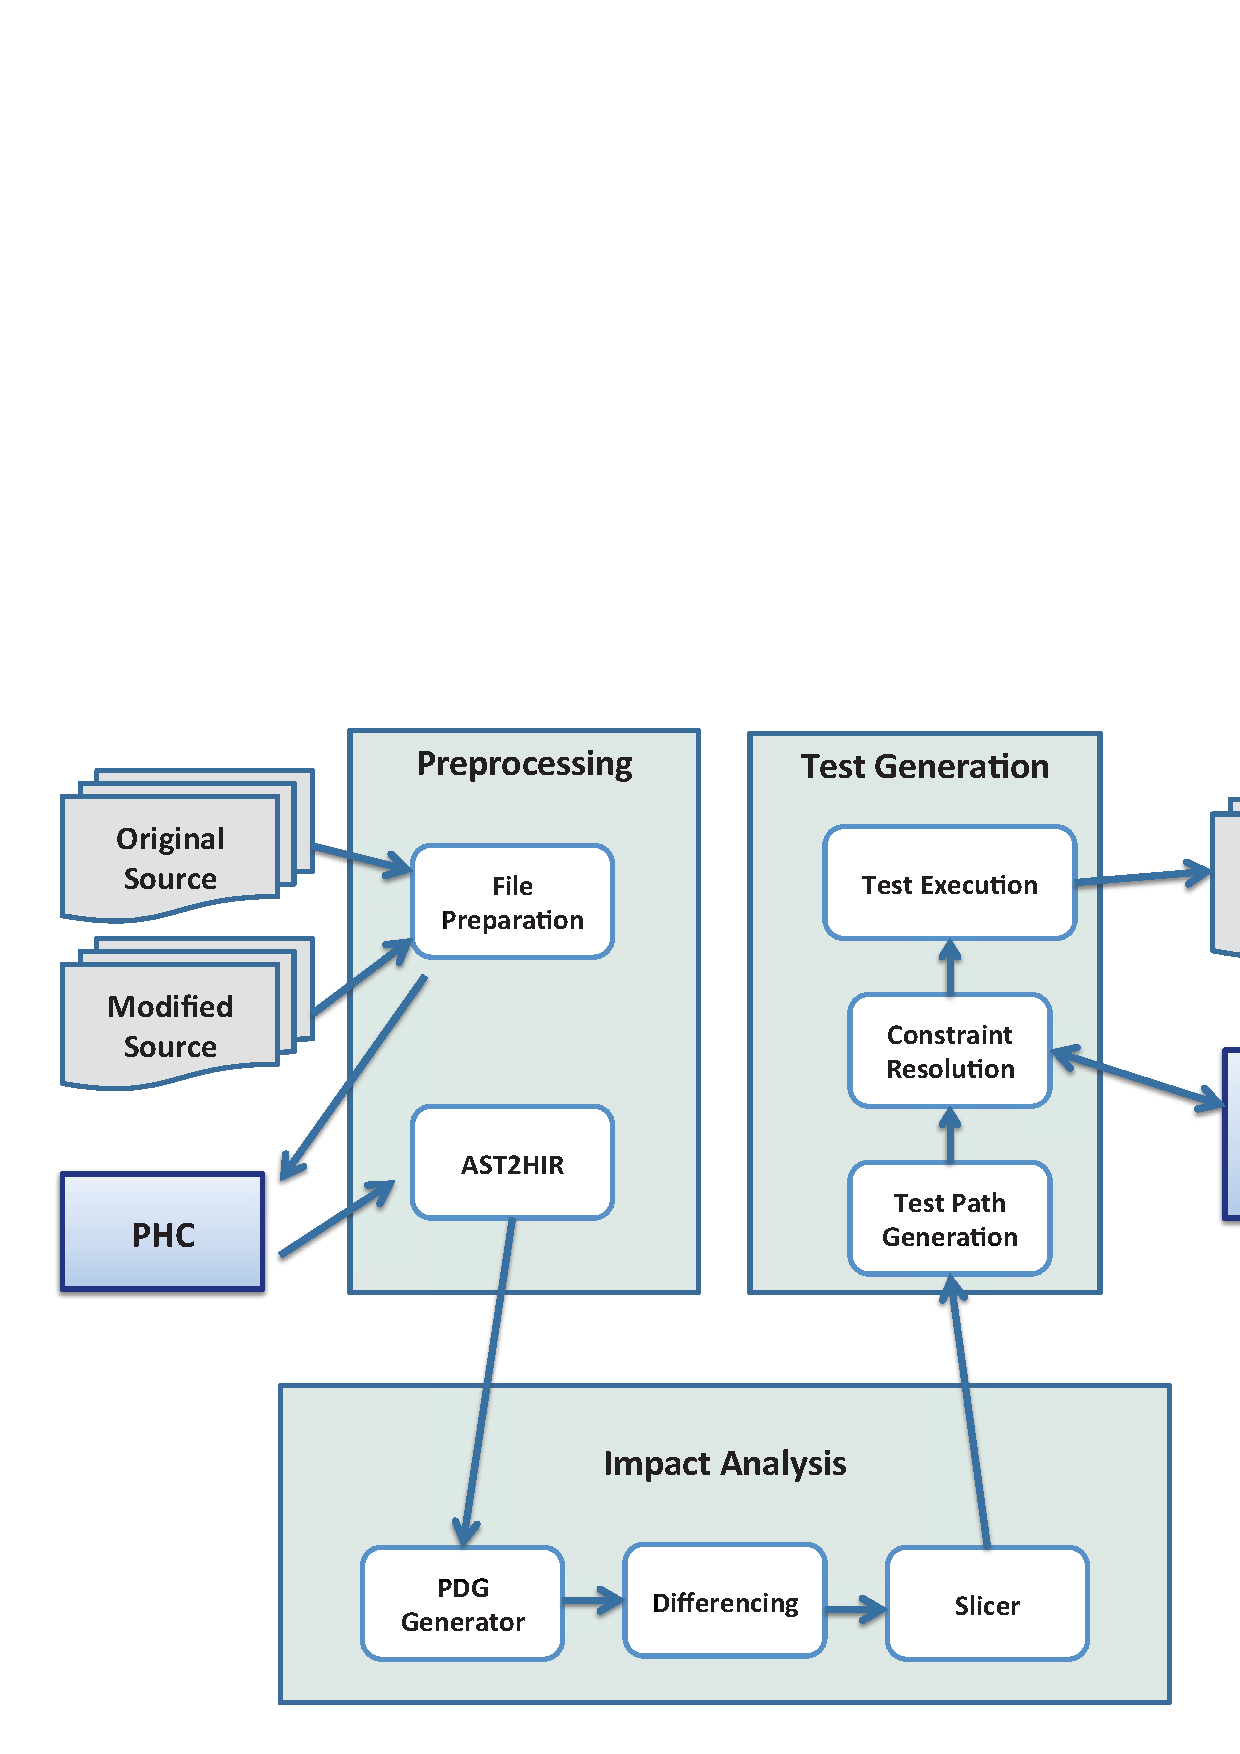
\includegraphics[width=0.8\columnwidth]{figures/parte-overview.pdf}
%%    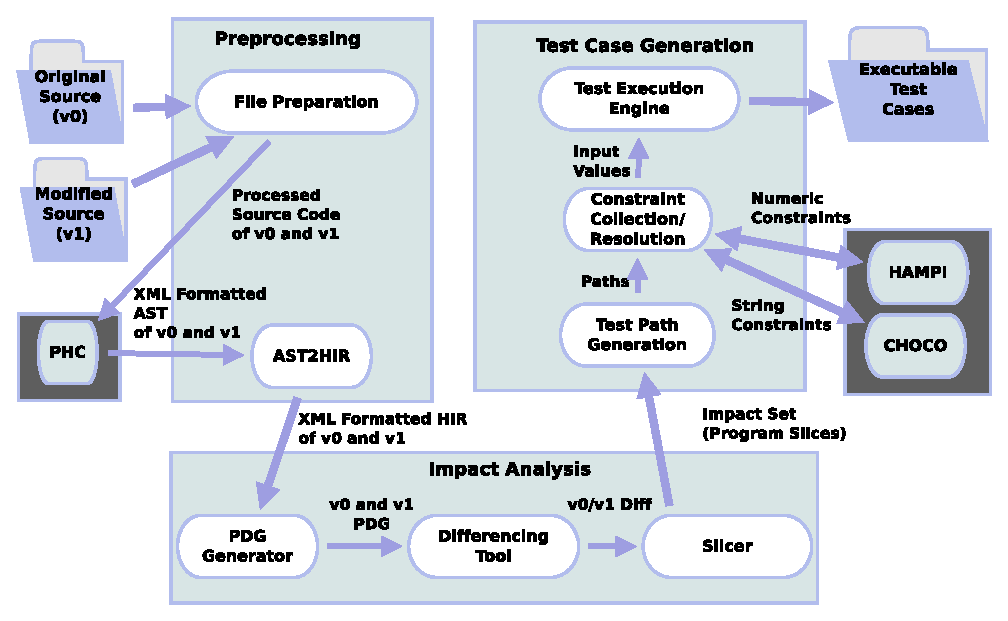
\includegraphics[width=0.8\textwidth]{figures/overview.eps}
%\vspace*{-40pt}
% \caption{Overview of PARTE} 
%\label{fig:overview}
%\end{figure*}
%
%Before we describe each activity in detail,
%we provide a brief overview of our approach.
%
%\begin{smallitem}
%\item {\bf Preprocessing} (the upper-left box in Figure~\ref{fig:overview}).
%In this step, PARTE converts abstract syntax trees (ASTs) generated by
%a PHP compiler, PHC~\cite{phc}, to high-level
%intermediate representation (HIR) that preserves variable
%names and converts this HIR back to ASTs.   
%
%\item {\bf Impact Analysis} (the lower box in Figure~\ref{fig:overview}).
%Using preprocessed files, a PDG (Program Dependence Graph) generator 
%builds PDGs for the two consecutive versions of a PHP web application. 
%Then, a differencing tool and a program slicer identify 
%the affected areas by the code changes (program slices).
%
%\item {\bf Test Case Generation} (the upper-right box 
%in Figure~\ref{fig:overview}).
%A test path generator creates test paths using program slices. 
%A constraint collector/resolver gathers string and numeric 
%input constraints, and resolves them using a constraint 
%solver, Choco~\cite{choco}.
%Finally, a test execution engine takes these resolved input 
%values, executes the application through Selenium~\cite{selenium},
%and records the test execution results.
%The last step is done manually because the current path 
%generator does not provide web elements for Selenium.
% 
%\end{smallitem}
%
%\input{ast.tex}
%\input{impact.tex}
%
\subsection{Test Generation}

%\begin{algorithm}[!b]
\vspace*{3pt}
%\begin{algorithm}[ht]
\caption{Path Generation}\label{fig:pathAlgol}
\begin{algorithmic}[1]
{\footnotesize
\State \textbf{Inputs:} \textbf{ \textit{slices[]}} \Comment{\textit{The slices
array contains all of the slices
that are generated by the analyzing changes made to the modified version of the application.}}
\State \textbf{Outputs:} \textbf{\textit{paths}} \Comment{\textit{An array of all of the linearly
independent paths produced from the set of slices.}} 
\State \textbf{Declare:} \textbf{\textit{edges}} \Comment{\textit{A set of edges traveled by the path 
generator}}
\State \textbf{\textit{currentPath}} \Comment {\textit{A placeholder for the path currently being
generator}}
\Procedure{PathGeneration}{$slices$}
	\State $paths \gets \emptyset$ 
	\State $edges \gets \emptyset$ 
	\For{$n \longleftarrow 0 $, $n < slices$.size(), $n$++}
	\While{$slices[n]$.size()$ > 0$}
		\State $currentNode \gets slice[n]$.firstNode()
	    \State $currentPath \gets \emptyset$ 
	    \State $currentPath$.add($currentNode$)
	    \State PDGTraverser($currentPath$, $paths$, $edges$, $slice[n]$, $currentNode$) 
	\EndWhile\label{mainPathWhile}
	\EndFor
	\State ResolvePaths();
	\State \textbf{return} $paths$
	\EndProcedure
}
\end{algorithmic}
\end{algorithm}

%%\begin{algorithm}[htb]
\begin{algorithm}[ht]
\caption{PDG Traverser}
\label{fig:walkpath}
\begin{algorithmic}[1]
{\footnotesize
\Procedure{PDGTraverser}{$currentPath$, $paths$, $edges$, $slice$, $currentNode$}
		
	\While{$currentPath$[lastNode].occursBefore($slice$.endNodes())}
		\If{$currentPath$.containsNoDiffNodes() $\wedge$ $currentPath$.cannotReachAdiffNode()}
		\State	\textbf{Return}
		\EndIf
		\If{$slice[n]$.contains($currentNode$)}
			\State $slice[n]$.remove($currentNode$)
		\EndIf
		\If{$currentPath$[lastNode].getExits.Size() $> 1$}	
			\For {$n \leftarrow currentPath$[lastNode].getExits.Size()-1,0,$n$--}
				\If {$currentNode$.exitEdge($n) \notin  edges$}
					\State $edges$.add($currentNode$.exitEdge($n$)
					\If {$n$ == 0}
						\State $curentNode \longleftarrow currentNode$.exit(n)
						\State $currentPath$.add($currentNode$);
						\State continue(2); \Comment{\textit{Go back to while loop}}
					\EndIf
					\State PDGTraverser($currentPath$.copy(), $paths$, $edges$, $slice$, $currentNode$.exit($n$))
				\Else
					\If{$currentNode$.exitEdge($n$) $\in currentPath$}
					\State $currentNode \longleftarrow$ findFirstNodeOutsideofLoop() 
					\EndIf
				\EndIf
					
			\EndFor 
		\Else
			\State $curentNode \longleftarrow currentNode$.exit(0)
			\State $currentPath$.add($currentNode$);
		\EndIf
	\EndWhile
	\If{$currentPath$[lastNode].isNotASliceEndNode()}
		\If {$currentPath$[lastNode].canReachASliceEndNode()}
			\State $currentPath$.findSliceEndNode();
		\Else
			\State \textbf{Return}
		\EndIf
	\EndIf
	\State $paths$.add($curentPath$)
\EndProcedure
}
%\vspace*{3pt}
\end{algorithmic}
\end{algorithm}

%
%In this phase, we need three steps:
%(1) test path generation, (2) input constraint collection
%and resolution, and (3) test execution.
%The following subsections describe each step in detail.
%  
%\vspace*{3pt}
%\subsubsection{Path Generation}
%
%The path generator creates linearly independent test paths 
%using the slices collected from the previous step.
%A {\em linearly independent path} is a path that includes 
%at least one edge that has not been traversed previously 
%(in a given set of paths under construction)~\cite{pressman}.
%
%Algorithms~\ref{fig:pathAlgol}
%show how to generate test paths using slices. The algorithm 
%is separated into two parts. The first part, 
%Algorithm~\ref{fig:pathAlgol}, iterates through and gathers 
%the nodes from the slice to use in the PDG traversing procedure. 
%The second part, Algorithm~\ref{fig:walkpath}, is the PDG 
%traverser which follows a subpath through the PDG using 
%the nodes in the slice as a guide. Algorithm~\ref{fig:pathAlgol} 
%begins by iterating through every remaining node in each slice.
%
%The PDG traverser (Algorithm~\ref{fig:walkpath}) begins 
%by analyzing a node in the PDG. If the node being 
%processed occurs after every node in the array of 
%remaining slice nodes (line 2), the PDG traverser checks 
%to see if the currently processed node can reach an end node 
%(a node where change propagation terminates) in the original 
%slice (lines 30 and 31). If the node can, it adds the path to 
%an end node of the current path (line 32). Otherwise, the path 
%is discarded (line 33).
%
%If the node that is being processed occurs
%before any of the end nodes in the slice, the node is 
%checked to see if it can reach the changed node (line 3). 
%If it cannot, the path is discarded.
%The PDG traverser then checks to see if a node is
%in the array of slice nodes. If it is, that
%node is removed from the array (lines 6 and 7).
%Every time the PDG traverser encounters a node with more than 
%one edge that has not been traversed, it creates a new subpath 
%that is a copy of itself for each of these edges and follows 
%them (lines 9-18). Once construction of the path has been 
%completed, the path is added to the path array (line 37).
%
%After subpath construction is finished, the first node 
%in a subpath is traced to an entry point for the program, 
%and the last node is traced to an exit point for the program 
%(line 16 of Algorithm~\ref{fig:pathAlgol}). 
%Algorithm~\ref{fig:pathAlgol} describes the basic construction 
%of these paths while omitting, for brevity, all special cases 
%that occur for cyclic graphs (loops and recursion).
%
%\subsubsection{Constraint Gathering and Resolution}
%
%Because the generated test paths contain only input parameters, not 
%actual input values, the input values need to be assigned to the 
%parameters to make test paths executable.
%The constraint collector collects constraints on input
%values needed to execute a particular program execution path.
%Its inputs are the outputs from the PDG generator and path
%generator. The top-level activities in the constraint collector
%are parsing the path and PDG XML files, generating constraints
%for each path, and writing the collected path constraints to
%an XML file. 
%
%Constraint collection begins with path nodes that contain
%a conditional statement. The primary activities to collect
%constraints are determining the truth value of conditional
%statements and reducing the conditional expression in these
%statements. 
%%A constraint is recorded only if it is not
%%a duplicate for a previously recorded constraint.
%A path constraint corresponds to a path PDG node with an
%``if'' statement. To determine the truth value of
%a constraint, the collector looks ahead one node in the
%path node list and examines the node type (which will be
%necessarily either \textit{true} or \textit{false}). After
%determining the constraint truth value, the constraint
%condition is then recursively reduced. Reduction of
%an expression involves parsing the expression string
%to determine the expression type (using regular expression
%matching), creating an expression object with this type,
%assigning any expression attributes from the parsed information
%(e.g., operator type) to the expression object, and generating
%appropriate expression objects for child expressions (if any).
%If there are child expressions, they are recursively reduced
%in the same way.
%
%Each type of expression provides its own method for reducing
%child expressions, in order to take advantage of information
%on the reduction context. For example, a compound boolean
%expression must have child expressions that are themselves
%boolean. When generating child expressions, this information
%can be provided, in addition to that which is provided by
%regular expression matching. This is useful in verifying
%that generated expressions are of the correct type.
%
%If regular expression matching determines an expression
%to be a variable (e.g., \$num\_of\_files), the reduction
%process involves additional steps:
%
%\begin{enumerate}
%  \item The collector backtracks in the path node list,
%starting at the index of the variable node. It continues
%backtracking until a PDG node is encountered that provides
%a definition of the variable, or until the beginning of
%the list is reached. In the case that a definition is found,
%the expression generated for the variable is of the complex
%variable type. This type is used for variables that can be
%defined in terms of other expressions. If, instead, no
%variable definition is found before reaching the start of
%the list, the expression generated is of the simple variable type.
%
%  \item Regular expression matching is performed on the
%variable expression string to determine if it is indexed
%(e.g., \$files[\$id]). These correspond to PHP array variables.
%An expression is then generated for the index of the array, and
%the generated expression for the variable is an indexed version
%of the type determined via backtracking (i.e., simple or complex 
%type).
%\end{enumerate}
%
%The recursive reduction process terminates on expressions of
%simple type, since simple type expressions do not contain
%child expressions that need to be reduced.
%After collecting a constraint, the collector records it for
%inclusion in the output. 
%%This step is only done if an equivalent
%%constraint is not already present in the list in order to
%%avoid outputting duplicate constraints. 
%Once all path constraints
%have been generated, the collector writes the constraint information
%in XML format. 
%
%The tool uses an existing constraint solver, {\em Choco},
%to determine the input values that satisfy the constraints
%for a given execution path (if such satisfaction is feasible).
%{\em Choco} is an open-source software and  consists of a set
%of libraries written in Java that provide many constraint solving
%features. It provides direct support for solving numeric and
%boolean constraints. We also use it to solve string constraints
%by mapping these constraints to equivalent constraints on integers. 
%Once all input values have been created, they are stored in XML file 
%format to be used later by the test execution engine.
%These files contain information about program paths and a list of input 
%variables for the paths. For each input variable, the variable type, 
%name, and value are given. 
%Resolving the inputs that use built-in PHP functions is not supported 
%by our tool, so those inputs require manual resolution. 
%Further, the constraint resolution tool sets the time limit for 
%input resolution, and it reports infeasible when it cannot find 
%the value within the time limit. Also, if the conditions for a 
%variable have conflict, the tool reports that case as infeasible.
%
%\subsubsection{Test Execution}
%
%Having assigned all input values to the parameters in the test 
%paths, we implemented a test execution engine that executes
%test cases over web applications using Selenium~\cite{selenium}.
%We used the Selenium WebDriver API (more specifically, the FirefoxDriver) 
%to set the web page elements according to the variable constraints for 
%the given execution path being tested. If test execution requires setup 
%logic, such as authentication, this is also performed using the WebDriver 
%API. Finally, the WebDriver API is used to execute the PHP file and the 
%results are passed to the test engine.
%As mentioned earlier, web elements are created manually becasue the current 
%path generator does not provide them.
%
%The reason that we have chosen to use the WebDriver API is that it allows us 
%to perform all the activities that will be required: finding and setting web 
%elements; performing any setup tasks required before the test case can be 
%executed (such as authentication); retrieving test execution results in the 
%HTML format.
%
%To give a better understanding of how the approach works, we use an e-commerce 
%example. Assume that we have two PHP files, login.php and add\_card.php, both 
%of which are accessed on different web pages. login.php contains the login 
%form that users can register/authenticate with, and add\_card.php allows 
%authenticated users to add their credit card information. Both login.php 
%and add\_card.php contain entry points for certain execution paths.
%
%If add\_card.php was modified between Version 1 and Version 2, we can run 
%the toolchain on this version pair and determine the constraints necessary 
%to test execution paths with entry points beginning in that file. Using 
%the Selenium WebDriver API, we can first access the login form contained 
%on login.php to register/authenticate the user. Afterwards, we use the 
%same API to directly execute add\_card.php, after initializing the values 
%of the web elements associated with path constraints. It would not be 
%necessary to start from login.php, since the PHP \$\_SESSION variables 
%used for authentication would still be valid during execution of add\_card.php, 
%regardless of the navigational path for arriving at this page. The results 
%of executing add\_card.php are recorded as an HTML file.
%
%
%\input{example-description.tex}

%
